\chapter{Motivation}
\label{ch:motivation}

Choosing a suitable topic for a Master's Thesis is not a readily decided matter. On one hand a student desires to show some insight into contemporary and maybe even complex problems, but on the other hand the task has to be achievable within a certain timeframe. The project should be theoretical enough to be of interest even for professors while at the same time (at least in Software Development) be practical enough to remaining motivating to the student. In the case of this Thesis I tried to combine scientific and engineering aspects into a project which could be expanded in future endeavors while keeping it sufficiently self contained to represent a work of its own.


\section{Scientific motivation}
\label{sect:scientific_motivation}

Having been a member of the HCI-KDD.org group for over 2 years now, I have developed a genuine interested in graph theory, machine learning, HCI as well as their applications in modern information systems - not least in the context of biomedical applications. Although finalizing my Master's study at a relatively advanced age, I am still open to pursuing a PhD in those areas. Therefore, it seemed logical to tackle some problems related to those fields; however significant progress in such matters are not easily achieved even by professional scientists, leave alone a single MSc student on a deadline...

For this reason I intended to contribute to the future work of Professor Holzingers Team by concerning myself with scientific matters without the pretension of being capable of improving on complex research efforts. As a result, I built on work already conducted in my Master's project by underpinning it with a more general and expandable Software architecture. Assisting (data) scientists by providing a better underlying infrastructure to accelerate their experimental iterations and making demanding processing steps available to researchers outside the field of computer science or software development, has been dubbed 'data engineering' over the recent years [article citations]. 

Popular projects like Apache Hadoop or Spark, Google's recently released TensorFlow and many other, more specialized clowd-based research platforms, fall under this category - albeit they boast very different properties and advantages and are therefore suitable for different, although overlapping, use cases. The Graphinius library (and future platform) presented in this thesis is unique in the sense that it allows computations directly on the client, but without requiring any installation, by utilizing a piece of software contained in any browser - the JavaScript virtual machine (JSVM). 


\section{Technological / engineering motivation}
\label{sect:technological_motivation}

As a student of Software Development and Business Management the two aspects of modern architectures and their repercussions on the next generation of business models are fascinating and of great importance to me. Especially the emergence of powerful JavaScript virtual machines in modern browsers as well as access to the GPU from inside a browser sandbox open up new opportunities for startup companies in many fields that were hitherto restricted to conservative Software Development paradigms. Physics simulations, machine learning tasks, the visualization and manipulation of complex data structures as well as console games can now be implemented on a general, ubiquitous platform without much loss of performance or usability. In the field of traditional Web applications, servers can act more and more as simple database-abstracting backends with near-zero computational and scalability requirements - especially if combined with cheap, global content delivery networks. On the other hand, handing much of the business logic over to the client side, an ever increasing complexity in cooperation between backend services, as well as emerging standards like websockets enabling realtime communication paradigms as publish/subscribe over traditional networking architecture also put challenges to a guild of developers used to write mainly server-side code such as Java, PHP or Ruby on Rails.

As a consequence, the following thesis is an attempt at merging my scientific curiosity with my drive towards new, exciting Software Development methodologies into a working, expandable prototype of a future Web based research platform. I am glad if I was partially able to live up to that goal.


\chapter{Introduction}
\label{ch:introduction}

The following sections shall give a brief introduction into how and why project Graphinius came into existence, what challenges we want to tackle building it, as well as the general objectives and potential new applications it might enable or make feasible in the future.


\section{What is Graphinius?}
\label{sect:intro_whats_graphinius}

Graphs are a fundamental tool of mathematics and can be applied to a very diverse field of modern scientific areas: network routing (information, traffic, logistics), social network / community analysis, image processing, NLP operating on graphs of document spaces and topic clusters as well as fraud detection via belief propagation networks (all of the mentioned and a few others will be described in Chapter 4).

A relatively novel addition to that spectrum is the emerging field of computational biology, in which we can find PPI, metabolics, or connectome graphs. Since BioMed Researchers are usually no tech experts, an intuitive, UI-based research platform could facilitate rapid experimental iterations. Graphinius aims to be such a Web-based, graph theoretical research platform offering real-time in-browser computations as well as tightly integrated visualization, interaction, and manipulation of graph structures. 

In this thesis I will mainly introduce GraphiniusJS and its underlying design principles; however, I am in the lucky position of already having supported the development of a graph visualization library in the context of a colleague's Master's Project. This WebGL / Three.js based library called GraphiniusVis uses low-level datastructures and concepts, enabling it to visualize up to 20k nodes / 60k edges inside a browser fluently even on middle-class laptops. I will also provide an outlook on the whole, emerging Graphinius platform and its exciting capabilities for researchers and students.


\section{The history of Graphinius}
\label{sect:ogma_history}
When I met Andreas Holzinger in November 2013 he presented me with a `crazy' idea, as he put it: To analyze dermatological images not by traditional image processing methods, but by first transforming them into a graph structure and subsequently apply graph mining algorithms with the goal of obtaining results at least comparable to the quality achievable as of date. My first experiments in what I quickly termed ``graph extraction'' from images' were conducted in Matlab and progressed rather modestly; being a developer used to employ C-style programing languages and Object oriented paradigms, Matlab seemed a peculiar (and very costly) way to perform specific, handwritten algorithms which did not lend themselves especially well to matrix representations and calculations. Moreover I was concerned with the fact that even if I succeeded in doing a great job in extracting usable graphs (what that meant was not clear to me at that time) I would not easily be able to share my work with colleagues outside the research community. Providing C++ / Java Code on Github for developers having working installations of those environments is certainly standard by today, but installations of Matlab (or Octave with specific add-on packages installed) are not widespread. Furthermore, in case my results would be interesting to the public as well, a live demonstration of the software at work might be desirable.

\par

After years of having utilizing Web based technologies and continuously researching new frameworks and improvements in that area, it seemed to me that if a whole document suite could be implemented in JavaScript (and even more demanding projects like an entire virtual machine inside the browser [CITE WEBSITE]), the time might be ripe to apply modern JavaScript Engines to the task of image as well as graph processing. Against my expectations Professor Holzinger did not have any objections and I was given green light to develop a simple prototype together with a colleague. This early work was focused purely on extracting graphs out of images without additional image preprocessing steps or subsequent graph analysis. As we would implement mathematical algorithms, we decided on TypeScript as a typed superset of JavaScript for our development process; no frameworks or numerical libraries were used. Within a little more than a month, we had an example website up and running which could load images into a canvas, segment them by either a Watershed or a Kruskal-based region merging algorithm and extract a graph from the label image; the results are available at http://berndmalle.com/imgextract and have been published in \cite{GraphExtractPaper}. As far as execution time was concerned, our crude and non-optimized JavaScript implementation fell just a little short of a comparable algorithm implemented in Matlab, with great upward potential for using in-browser optimizations or even GPU-accelerated processing.

\par

Of course there were downsides too - JavaScript engines are naturally single-threaded even in 2015, so long-running intense computing tasks tend to block other functions. This is even true for other Browser-intern modules like the rendering engine or input event handling, so that the whole user experience is severely diminished when computing demanding operations. However, a possibility to avert this behavior is the usage of WebWorkers which have been introduced as a working draft as early as 2009, but until recently haven't been widely supported. Also, possible downsides to their usage in situations where large datastructures need to be copied from the main thread to a worker (and back) have to be considered. More interestingly though, it became clear early on that implementing our suite of algorithms as a Web based platform would bring with it several major advantages over traditional software approaches amongst which are easy reproducability, effortless scalability and online meta machine learning opportunities; all of those advantages will be discussed in detail in subsequent chapters.

\par

Building upon those insights Professor Holzinger and I came up with a project called iKnodis.net - Interactive Knowledge Discovery in Networks) - which was designed to cover the whole processing pipeline from image preprocessing over graph extraction to graph analysis and result visualization. In the process of defining those modules it became clear that single components of the processing pipeline would have to be interchangable so that other students be able to contribute new algorithms from future student and research projects to the different stages of operations. This generated the challenge of coming up with a flexible pipelining architecture that would itself be aware of the pre/postconditions in each stage of computation and upon satisfaction of all the constraints be able to connect the different parts together as well as executing them utilizing Webworkers in the background. On this basis I realized another potential advantage of a Web based research platform: by affording users the opportunity to contribute their own algorithms for certain parts of the pipeline via file upload, it would be possible to gather a large collection of algorithms in a much shorter period of time as compared to researchers working in isolated teams.

\par

\begin{figure}[ht]
	\label{fig_iKNOdis_structure}
	% \centering
	% \hspace*{-0.5cm}
	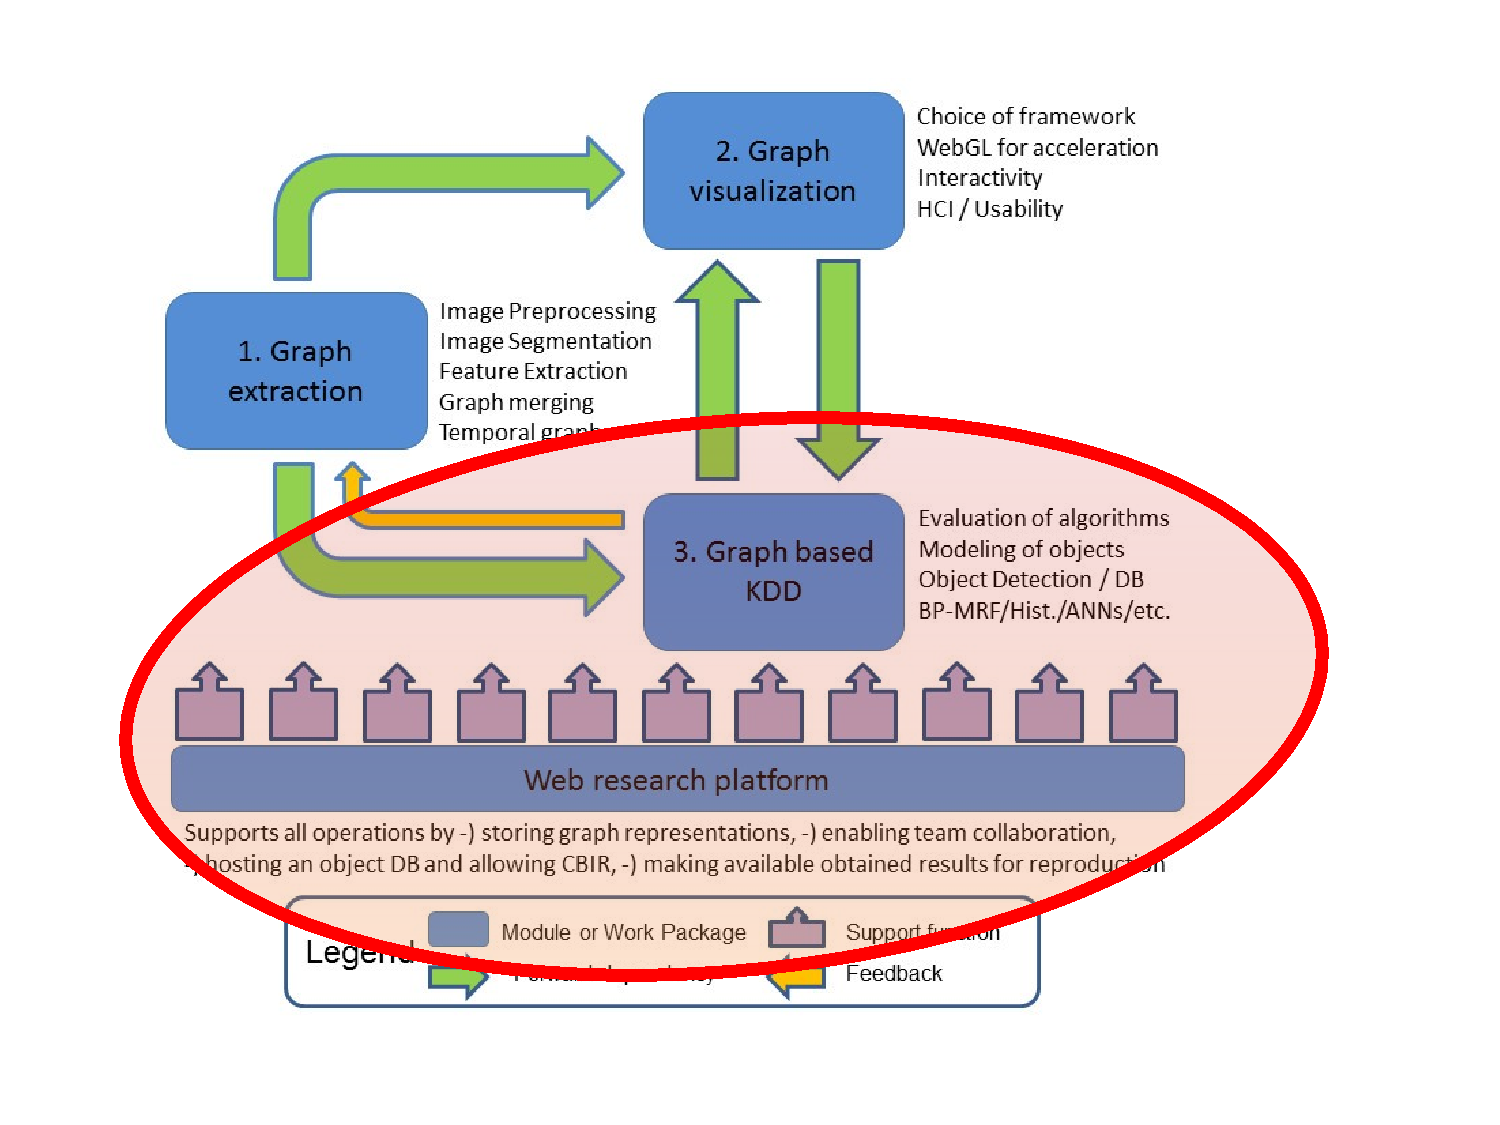
\includegraphics[width=1.1\textwidth]{figures/iKNOdis_OGMA_structure}
	\caption{Former project iKNOdis architecture overview}
\end{figure}


In the process of creating an FWF proposal out of iKnodis, the project was split into two separate projects in order to make them amenable to independent smaller funding efforts as well as different groups of developers working on their respective areas of interest yet maintaining their focus towards achieving the common goal. This resulted into iKNOdis now spanning graph extraction out of images as well as 3-dimensional visualization of the resulting graph structures via a Browser based method. 

The remaining modules of building a Web Based research platform as well as establishing graph mining algorithms able to tackle object recognition / image classification tasks usually covered by traditional image processing techniques, have been outsourced to project OGMA, the Open Graph Mining Architecture. Although it will be in the context of OGMA that this Master Thesis will play out, the resulting smart computational pipeline will also encompass the algorithms of iKNOdis. Indeed, a graph extraction algorithm already implemented during my Master's Project \cite{GraphExtractPaper} will be part of the test cases for the practical implementation found in later chapters of this work. 

\section{How this thesis is structured}
\label{section:thesis_structure}

The rest of this chapter is composed of a short description of how composite machine learning tasks are handled today followed by the question if a transition towards Web based technologies is feasible given the narrow implementation choices in that field. We will then explore in detail what benefits researchers as well as the whole research community could derive from conducting experiments on such a platform; therefore we have to outline potential properties and focal points of such a technology. Upon a short discussion of how the gathering of metadata about diverse ML/KDDM experiments as well as their results could open up new opportunities, we will envision a future recommender system for composing machine learning pipelines based on a heuristic approach. This chapter will close with a brief overview of the general properties of the smart computational pipeline (henceforth called ``SCP'') under development.

\par

Chapter 3, ``Related work'', will consider past and present approaches to recognizing objects in images as well as conduct image classification utilizing graph based approaches and will therefore show the validity of OGMA's objectives. Furthermore, contemporary efforts of building machine learning pipelines as well as the data and insights they are based on will be investigated. An overview of existing software solution will conclude chapter 2.

\par

In Chapter 4, ``SCP General Design'', we will lay the technical and scientific foundation for the design of a smart computational pipeline for OGMA. Building upon a high level overview of machine learning pipelines and their different stages in theory, we will be able to derive general requirements that any piece of software handling those processes will have to fulfill. Further, the question will arise as to how to represent algorithmic ``packages'' for the sake of this undertaking and how dependencies in the I/O of each pipelining stage should be resolved automatically. Following an analysis of how to use existing package manager algorithms to fulfill those requirements, the question of executing a valid processing pipeline within a browser environment considering modern users' expectations of fluidity and asynchronicity will be dealt with. At the end of this chapter, we will propose a data model for storing the experiment metadata for further analysis and find a description of the algorithms used for testing the pipeline later on.

\par

The next chapter 5, ``SCP Software Design'', will elaborate on the actual software implementation as well as the software development process followed in this project. First a set of requirements for modern Web based software will be compiled; based on this checklist an exploration of possible suitable technologies for both server and client will be conducted and their respective strenghts and weaknesses revealed. After a detailed comparison I will argue for the particular combination of choices I made and will subsequently describe the development process used to implement the pipeline. An illustration of how Webworkers were used to execute the pipeline as well as how results were visualized will finalize this chapter.

\par

The 6th chapter on ``Results and Discussion'' will wrap up the efforts undertaken in this project. I will first go into details about the project implementation and the difficulties and / or caveats that arose during my work. A detailed experimental setup will be described and the expected behavior of the SCP defined, while the ensuing section should verify those expectations and therefore validate the approach taken. A discussion of open and interesting challenges as well as  an outlook on future possibilities to enhance and expand on this work will top of this chapter.

\par 

Eventually the 7th and last chapter, ``Conclusion'', will give a short recap on the motivation, goals, and main issues of this project and thus bring the thesis to its completion.



\section{How Machine Learning / KDDM are approached today}
\label{sect:ml_kddm_today}

When taking the famous Machine Learning MOOC tought by Prof. Andrew Ng from Stanford University on Coursera in 2013, one story he was conveying during a section on optimizing Machine Learning Pipelines had especially caught my attention. As a specialist in high demand Prof. Ng is frequently consulting for Silicon Valley companies in matters of Machine Learning and Artificial Intelligence. On one of these occasions, the client company had been trying to optimize their ML pipeline for the better parts of 2 years without any significant improvements in their results. After looking at the different stages of their pipeline and conducting a so-called ceiling analysis, Prof. Ng concluded that two developers had spent 18 months on optimizing their background separation algorithm while the most significant potential for improvement really lay in a latter stage of the process. Based on this analysis the company was able to remedy the shortcomings in a relatively short amount of time.

\par

This incident shows how much effort is potentially squandered by trying to implement sophisticated processing pipelines within isolated teams in a non-standardized fashion: Proprietary approaches - both in technology as in methodology - hinder the exchange of information with other members of the research community, thus opening up vulnerabilities to making mistakes which could have easily been avoided by considering the experience of other professionals. The following properties of data analysis / ML projects seem to give rise to such vulnerabilities:

\begin{itemize}
	\item \textbf{Isolation.} Working on common machine learning problems in isolated teams without communication makes comparison of approaches as well as results unnecessarily hard. Dealing with errors at any stage of the pipeline takes more effort than necessary due to a lack of reference values, while achieving superb results has little to no effect on the potential of other experts.
	\item \textbf{Proprietary Software.} Countless professionals prefer developing data analysis pipelines in highly proprietary software environments like Matlab or Mathematica. This prevents an influx of solid, community-tested algorithms while preventing others from gaining knowledge acquired in such organizations (if they are unwilling to pay for the software).
	\item \textbf{Irreproducibility.} As unpublished code cannot be perfectly reverse engineered, experiments conducted in isolation can't be easily corroborated. This might be advantageous with respect to product development and patent procedures, but is usually detrimental to the efforts of researchers trying to get published and spreading their insights.
	\item \textbf{Lack of scalability.} Last but not least, heterogeneous and highly customized data processing pipelines might not lend themselves well to parallelization, which might prevent the use of such algorithms on quickly expanding datasets.
\end{itemize}


Papers to cite in this context: \\
\cite{LargeScaleMLPipelines}
\cite{MLPipelineMLlib}
\cite{DataAnalysisDSWorkflow}
\cite{StanfordNLP}
\cite{MLPipelines}
\cite{Make2013}
\cite{AnalLifecycle}
\cite{DataScienceTools2013}
\cite{AnalOneComponent2013}


\section{A Web based approach - why?}
\label{sect:web_transition}

\section{How a Web based approach could benefit users, researchers and society}
\label{sect:web_benefits}

\begin{itemize}
	\item \textbf{Ease of access.}
	\item \textbf{Effortless scalability.}
	\item \textbf{Built-in potential analysis.}
	\item \textbf{Server Side Meta Machine Learning.} As researchers start using our platform, their pipeline configurations, input descriptions, task specifiers (classification, text analysis etc.) as well as results will be stored on the server. Enough data provided, such a database might be amenable to the development of heuristics on the expected success of a particular algorithm invoked at a specific stage of the pipeline.
	\item \textbf{Heuristics-based recommendations.} Based on the last section, an optimal pipeline configuration might be computed provided only the input data (image, text, point cloud etc.) as well as the desired result. The Smart Computational Pipeline would then self assemble (given the user has no objections) and immediately commence the experiment.
\end{itemize}



\section{General applications}
\label{sect:ogma_focal_points}

\subsection{education}
\label{ssect:education}

\subsection{algorithm prototyping}
\label{ssect:algo_proto}

\subsection{research platform}
\label{ssect:research}

